\chapter{Geodesics}\label{chap4:chap4}

\section{The  first variation}\label{chap4:sec1}\pageoriginale

In this article, we study the 
following question; given two points $m$, $n$ in an r.m.\@ $(M,g)$,
look for a curve $f$ with end points $m$, $n$ which has minimal
length among all curves in $M$ with end points $m$, $n$. Then the
first variation has to be zero for all one-parameter families of
curves with fixed ends $m$, $n$. This will lead us to a {\em
sufficient} condition involving the acceleration vector $f''$ of
$f$ and from there to a spray on $(M,g)$ canonically, so to
geodesics in $(M,g)$. The necessity of this condition could be
proved directly but we will not do it, for it will be a consequence
of Chapter VII. We shall, in the course of these considerations,
obtain a useful formula for a geodesic in $(M,g)$, the first
variation formula.

\quad 
Let us consider an r.m.\@ $(M.g)$ and two points $m$, $n\in M$; let
$f$ be a one-parameter family of curves, for which we use the notation
introduced in (\ref{chap2:sec8}). We suppose that $f:(I=]-\epsilon$,
  $1+\epsilon[\,)\times J\to M$ with $0\in J$ and $\epsilon>0$;
    moreover we suppose that $||f'_{0}(t)||-1 \, \forall t$.

For the lengths of the $f_{s}$'s we define the {\em first variation}
$l'(0)$ by:
\begin{equation*}
l'(0)=\frac{d}{ds}(lg(f_{s}|[0,1]))_{s=0}.\tag{4.1.1}\label{chap4:4.1.1}
\end{equation*}
To compute $l'(0)$, if $\alpha$ is the canonical form on $T(M)$
(definition in (\ref{chap3:3.6.5}), we set
\begin{equation*}
\beta=\uub{P}^{\ast}(\alpha).\tag{4.1.2}\label{chap4:4.1.2}
\end{equation*}\pageoriginale 
We have:
\begin{equation*}
E\circ\uub{P}=\alpha(\uub{P}^{T}\circ P)=\beta(P);\tag{4.1.3}\label{chap4:4.1.3}
\end{equation*}
for, $\alpha(\uub{P}^{T}\circ P)=g(p'\circ\uub{P}^{T}\circ
P,P^{T}\circ \uub{P}^{T}\circ P)$. But $p'\circ\uub{P}\circ P=\uub{P}$
and $p^{T}\circ \uub{P}\circ P=\uub{P}$.

Since $||f'_{0}(t)||=1$ we have, by the very definition of
$Q=\dfrac{\partial}{\partial s}$, the following commutative diagram:
\[
\xymatrix@C=2.5cm@R=1.5cm{
 & T(T(M))\ar@<.25em>[d]^{p^{T}}\ar@<-.25em>[d]_{p'}\\
T(I\times J)\ar[r]^{f^{T}}\ar[ur]^{\uub{P}^{T}} & T(M)\ar[d]^{p}\\
I\times
J\ar@<.25em>[u]^{P}\ar@<-.25em>[u]_{Q}\ar@<.25em>[ur]^{\uub{Q}}\ar@<-.25em>[ur]_{\uub{P}}\ar[r]_{f}
& M
}
\]
Further,
\begin{align*}
lg(f_{s}|[0,1])=\int\limits^{1}_{0}||f'_{s}(t)||\dt&=
\int\limits^{1}_{0}(E\circ \uub{P})^{\frac{1}{2}}(t,s)\dt=\\
&=\int\limits^{1}_{0}\beta(P)^{\frac{1}{2}}(t,s)\dt,
\end{align*}
and
\begin{align*}
l'(0)&=Q(\int\limits^{1}_{0}(\beta(P))^{\frac{1}{2}}(t,s)\dt)\\ 
&=(1/2)\int\limits^{1}_{0}Q(\beta(P))(t,0)\cdot(\beta(P)(t,0))^{-1/2}\dt=\\
&=(1/2)\int\limits^{1}_{0}Q(\beta(P))(t,0)\dt.
\end{align*}
But\pageoriginale
$$
d\beta(P,Q)=P\beta(Q))-Q(\beta(P))-\beta([P,Q])\quad\text{and}\quad [P,Q]=0
$$
so we get
$$
l'(0)=(1/2)\int\limits^{1}_{0}P(\beta(Q))(t,0)\dt-(1/2)\int\limits^{1}_{0}d\beta(P,Q)(t,0)\dt.
$$
From the definition $P=\dfrac{\partial}{\partial t}$:
$$
\int\limits^{1}_{0}P(\beta(Q))(t,0)\dt=[\beta(Q)]^{1,0}_{(0,0)}
$$
but
\begin{align*}
\beta(Q)=\alpha(\uub{P}^{T}\circ Q)=(\text{see (\ref{chap3:3.6.6})}) &=
g(p'\circ\uub{P}^{T}\circ Q,p^{T}\circ \uub{P}\circ Q)=\\
&= g(\uub{P},\uub{Q})\text{ to the effect:}
\end{align*}
\begin{equation*}
l'(0)=(1/2)[g(\uub{P},\uub{Q})]^{(1,0)}_{(0,0)}-(1/2)\int\limits^{1}_{0}d\beta(P,Q)(t,0)\dt.\tag{4.1.4}\label{chap4:4.1.4} 
\end{equation*}
We can also write it as:
\begin{equation*}
l'(0)=(1/2)[g(\uub{P},\uub{Q})]^{(1,0)}_{(0,0)}-(1/2)\int\limits^{1}_{0}d\alpha(f''_{0}(t),(\uub{P}^{T}\circ Q)(t,0))\dt\tag{4.1.5}\label{chap4:4.1.5}
\end{equation*}
for the acceleration $f''_{0}(t)$ of $f_{0}$ (see (\ref{chap0:0.5.8})).

Clearly:

\setcounter{section}{1}
\setcounter{subsection}{5}
\subsection{}\label{chap4:4.1.6}
If $f(0,s)=m$ and $f(l,s)=n\forall s\in J$, then
$$
\left[g(\uub{P},\uub{Q})\right]^{(1,0)}_{(0,0)}=0.
$$

But this does not imply that $f''_{0}(t)$ should be such that
$i(f''_{0}(t))(d\alpha)=0$ for $\uub{P}^{T}\circ Q(t,0)$ is not an
arbitrary element in $T(T(M))$. For, adding (\ref{chap0:0.5.9}),
(\ref{chap3:3.6.10}) and (\ref{chap3:3.1.8}) we get:

\subsection{}\label{chap4:4.1.7}\pageoriginale
if $z$ vertical then $(d\alpha)(f''_{0}(t),z)=-(1/2)z(E)$.

But $(\uub{P}^{T}\circ Q)E=Q(\beta(P))$ so we have
\begin{align*}
&(i(f''_{0}(t))(d\alpha)+(1/2)dE)(\uub{P}^{T}\circ Q)(t,0)\\ 
&=(P(\beta(Q))-Q(\beta(P))+(1/2)Q(\beta(P)))(t,0)=\\
&=(P(\beta(Q))-(1/2)Q(\beta(P))(t,0)
\end{align*}
and finally:
\begin{equation*}
l'(0)=[g(P,Q)]^{(1,0)}_{(0,0)}-\int\limits^{1}_{0}((i(f''_{0}(t)(d\alpha)+(1/2)dE))(\uub{P}^{T}\circ
Q)(t,0)\dt\tag{4.1.8}\label{chap4:4.1.8} 
\end{equation*}
from which we get:

\setcounter{subsection}{8}
\subsection{$i(f''_{0}(t)(d\alpha)+(1/2)dE=0$ is a sufficient
  condition for $f_{0}$ to be of critical length among all curves with
ends $m$, $n$.}\label{chap4:4.1.9}

And in particular

\subsection{}\label{chap4:4.1.10}
if the curve $f_{0}$ is such that $i(f''_{0})(d\alpha)+(1/2)dE=0$ then
we have the {\em first variation formula}:
$l'(0)=[g(\uub{P},Q)]^{(1,0)}_{(0,0)}$.

We are so lead to the following:

\section{The canonical spray on an r.m.\@ $(M,g)$}\label{chap4:chap4-sec2}

By Proposition (\ref{chap3:3.6.8}) it follows that there exists one and
only one $G\in\mathscr{C}(T(M))$ such that
\begin{equation*}
i(G)(d\alpha)=-\frac{1}{2}dE.\tag{4.2.1}\label{chap4:4.2.1}
\end{equation*}

Regarding the $G$ we prove the following proposition.

\setcounter{subsection}{1}

\subsection{}\label{chap4:4.2.2}

\begin{prop*}
$G$ is a spray on $M$.
\end{prop*}

\begin{proof}
First let us prove that $p^{T}\circ G=\id_{T(M)}$. For any $x\in T(M)$
and $z\in V_{x}$ we have, on the one hand, by (\ref{chap3:3.1.8})
$$
(d\alpha)(G(x),z)=-\frac{1}{2}z(E)=-g(x,\xi(z))
$$\pageoriginale
and, on the other by (\ref{chap3:3.6.10})
$$
(d\alpha)(G(x),z)=-g({}^{T}(G(x)),\xi(z))
$$
and hence
$$
g(p^{T}(G(x))-x,\xi(z))=0.
$$
Since $\xi$ is an isomorphism between $V_{x}$ and $T_{x}(M)$ and $g$
is non - degenerate we have
$$
p^{T}(G(x))=x,\forall x\in T(M).
$$
Now let us prove the homogeneity.
\end{proof}

First let us note that
$$
\alpha\circ h^{T}_{\theta}=\theta\cdot \alpha,
$$
In fact, $\forall z\in T(T(M))$ we have:
\[
\xymatrix@R=1.2cm@C=2.5cm{
T(T(M))\ar[r]^{h^{T}_{\theta}}\ar@<.25em>[d]^{p^{T}}\ar@<-.25em>[d]_{p'}
& T(T(M))\ar@<.25em>[d]^{p^{T}}\ar@<-.25em>[d]_{p'}\\
T(M)\ar[r]^{h_{\theta}}\ar[d]_{p} & T(M)\ar[d]^{p}\\
M\ar[r]_{\id_{M}} & M
}
\]
\begin{align*}
\alpha(h^{T}_{\theta}(z)) &= g(p^{T}(h^{T}_{\theta}(z)),p'\circ
h^{T}_{\theta}(z))=\\
&= g((p\circ h_{\theta})^{T}(z),h_{\theta}\circ
p'(z))=g(p^{T}(z),\theta\cdot p'(z))=\\
&=\theta g(p^{T}(z),p'(z))=\theta\cdot\alpha (z).
\end{align*}\pageoriginale

Hence, we have, for every $z$, $z'$ in $T(T(M))$,
$$
d\alpha(h^{T}_{\theta}(z),h^{T}_{\theta}(z'))=\theta\cdot
d\alpha(z,z').
$$

Now for any $Z\in\mathscr{C}(T(M))$ we have
\begin{align*}
d\alpha(\theta(h^{T}_{\theta}\circ G), h^{T}_{\theta}\circ Z) &=
\theta\cdot d\alpha(h^{T}_{\theta}\circ G,h^{T}_{\theta}\circ Z))\\
&= \theta^{2}\cdot d\alpha(G,Z)=-\frac{1}{2}\theta^{2}\cdot
Z(E),\text{ \ and also}
\end{align*}
\begin{align*}
d\alpha(G\circ h_{\theta},h^{T}_{\theta}\circ Z)
&=-\frac{1}{2}h^{T}_{\theta}\cdot Z(E)\\
&=-\frac{1}{2}Z(E\circ h_{\theta})=-\frac{1}{2}Z(\theta^{2}\cdot
E)=-\frac{1}{2}\theta^{2}\cdot Z(E).
\end{align*}
Again, as above, since $d\alpha$ is non-degenerate we have
$$
G\circ h_{\theta}=\theta(h^{T}_{\theta}\circ G).
$$
Now we give the following definition.

\subsection{}\label{chap4:defi4.2.3}

\begin{defi*}
The spray $G$ of the above proposition is called {\em the canonical
  spray of the} r.m.\@ $(M,g)$.
\end{defi*}

Whenever we talk of a spray on an r.m.\@ we always mean the canonical
spray. In view of this we can talk of {\em geodesics on an} r.m.

By the definition of isometry $E$ is invariant under isometry and by
(\ref{chap3:3.6.7}), $d\alpha$ is also invariant under isometry and we have
the following:

\subsection{}\label{chap4:4.2.4}

\begin{prop*}
If\pageoriginale
$$
\lambda:(M,g)\to (N,h)
$$
is an isometry, and ${}^{M}G$ (respectively ${}^{N}G$) is the
canonical spray of $(M,g)$ (respectively on $(N,h)$) then
$$
{}^{N}G=(\lambda^{T})^{T}\circ {}^{M}G\circ(\lambda^{-1})^{T}.
$$
\end{prop*}

\begin{proof}
Let any $Z'\in\mathscr{C}(T(N))$; since $\lambda$ is an isometry and
hence in particular, a diffeomorphism, there exists a
$Z\in\mathscr{C}(T(M))$ such that $Z'=(\lambda^{T})^{T}\circ Z\circ
(\lambda^{-1})^{T}$. Set moreover:
$$
G'=(\lambda^{T})^{T}\circ {}^{M}G\circ(\lambda^{-1})^{T}.\text{
  \ Then, by ((\ref{chap3:3.6.7})), \eqref{chap0:0.2.6}, (\ref{chap0:0.2.9}),}  
$$
we have:
\begin{align*}
(i(G')\cdot d({}^{N}\alpha))(Z') &=
d(((\alpha^{-1})^{T})^{\ast}(M\alpha))(G',Z')=\\
&= ((\lambda^{-1})^{T})^{\ast}(d({}^{M}\alpha))(G',Z')=\\
&= d({}^{M}\alpha)(((\lambda^{-1})^{T})^{T}\circ G'\circ
\lambda^{T},((\lambda^{-1})^{T})^{T}\circ Z'\circ \lambda^{T})\\
&= d({}^{M}\alpha)(G',Z')=(i({}^{M}G)\cdot d({}^{M}\alpha))(Z).
\end{align*}
\end{proof}
Now, by the definition of ${}^{M}G$ and because $\lambda$ is an
isometry implies $M$ ${}^{M}E={}^{N}E\circ\lambda^{T}$, we have:
\begin{align*}
(i({}^{M}G)\cdot d({}^{M}\alpha))(Z)=-\frac{1}{2}d({}^{M}E)(Z) &=
  -\frac{1}{2}d({}^{N}E)((\lambda^{T})^{T}\circ Z\circ
  (\lambda^{-1})^{T})=\\
&=-\frac{1}{2}d({}^{N}E)(Z').
\end{align*}

\subsection{}\label{chap4:4.2.5}



\begin{coro*}
If $\lambda:(M,g)\to (N,h)$ is an isometry and $f$ a geodesic in
$(M,g)$, then $\lambda\circ f$ is a geodesic in $(N,h)$. 
\end{coro*}

\begin{proof}
Let\pageoriginale $(I,f)$ be an integral curve of ${}^{M}G$ in
$T(M)$. Then $(I,\lambda^{T}\circ f)$ is an integral curve of
${}^{N}G=(\lambda^{T})^{T}\circ {}^{M}G\circ(\lambda^{-1})^{T}$ in $T(N)$.
\end{proof}
For:
\begin{align*}
(\lambda^{T}\circ f)' =(\lambda^{T}\circ f)^{T}\circ P &=
  (\lambda^{T})^{T}\circ f'=(\lambda^{T})^{T}\circ {}^{M}G\circ f=\\
&= ({}^{N}G\circ \lambda^{T})\circ f={}^{N}G\circ (\lambda^{T}\circ f)'.
\end{align*}

\subsection{}\label{chap4:4.2.6}

\begin{coro*}
If $\lambda:(M,g)\to (N,h)$ is an isometry, then
$\lambda^{T}({}^{M}\Omega)={}^{N}\Omega$ and the following diagram is
commutative:
\[
\xymatrix@C=2.5cm@R=1.5cm{
M_{\Omega}\ar[d]_{M_{\exp}}\ar[r]^{\lambda^{T}} &
N_{\Omega}\ar[d]^{N_{\exp}}\\
M\ar[r]^{\lambda} & N
}
\]
\end{coro*}

\begin{proof}
Apply (\ref{chap1:1.4.5}).
\end{proof}

We slightly generalize the above results in the:

\subsection{}\label{chap4:4.2.7}

\begin{prop*}
Let $(M,g)$ and $(N,h)$ be two r.m.'s of the same dimension and a map
$\lambda\in D(M,N)$ be such that $\lambda^{\ast}h=g$. Then $\lambda$
is a local isometry; moreover, if $(I,f)$ is a geodesic in $(N,h)$ and
$\widehat{f}:I\to M$ such that $\lambda\circ\widehat{f}=f$, then
$\widehat{f}$ is a geodesic in $(M,g)$.
\end{prop*}

\begin{proof}
We note first the injectivity of $\lambda^{T}_{m}\forall m\in M$,
which comes from $\lambda^{\ast}h=g$ and $g$ positive definite; the
equality of dimensions then implies $\lambda^{T}_{m}$ is an
isomorphism $\forall m\in M$; hence the inverse function theorem and
$\lambda^{\ast}h=g$ imply the local isometry.
\end{proof}

\begin{remark*}
\ref{chap4:4.2.7} can \pageoriginale be applied, in particular, to a riemannian {\em
  covering}. 
\end{remark*}

\subsection{}\label{chap4:4.2.8}

\begin{example*}
Let us determine the canonical spray of $(\mathbb{R}^{d},\epsilon)$.
\end{example*}

First of all from the definition of the scalar product of $g$ we can
identify $\alpha$ and $\mu$, and $d\alpha$ and $d\mu$. Now by
\eqref{chap0:0.4.26} we have, for every $z$, $z'$ of $T(M)$,
$$
d\alpha(z,z')=(\zeta^{T}(z))\cdot (p^{T}(z')-(\zeta^{T}(z))\cdot (p^{T}(z)),
$$
and hence $\forall x\in T(M)$ we have
\begin{align*}
d\alpha (G(x),z) &= (\zeta^{T}(G(x)))\cdot
(p^{T}(z))-(\zeta^{T}(z))\cdot (p^{T}(G(x)))=\\
&= (\zeta^{T}(G(x)))\cdot (p^{T}(z))-\zeta^{T}(z)\cdot \zeta(x).
\end{align*}
On the other hand
$$
E(x)=(\zeta(x))\cdot (\zeta(x)),
$$
and hence for $z\in T_{x}(T(M))$, by (0.4.5)
$$
z(E)=2(\zeta(x))\cdot(\zeta^{T}(z)).
$$
Hence
$$
(\zeta^{T}\circ G(x))\cdot p^{T}(z)=0,\forall z\in T_{x}(T(M)).
$$
But since $g$ is non-degenerate and $p^{T}$ is onto $T_{x}(M)$ we have
\begin{equation*}
\zeta^{T}(G(x))=0.\tag{4.2.9}\label{chap4:4.2.9}
\end{equation*}
Consequently, by (\eqref{chap2:2.1.22}), the geodesics are segments of
straight lines. A more geometrical proof would be to use the symmetry
around a line in $\mathbb{R}^{d}$ (which is an isometry) and apply the
local uniqueness of geodesics and the lemma (\ref{chap4:4.2.6}). We
shall do this in a more general situation in \S 4.

\section{First consequences of the definition}
\label{chap4:chap4-sec3}\pageoriginale

\subsection{}\label{chap4:4.3.1}

\begin{prop*}
$G(E)=0$.
\end{prop*}

\begin{proof}
In fact, by definition, we have
$$
G(E)=(dE)(G)=-2d\alpha(G,G)=0.
$$
\end{proof}

\subsection{}\label{chap4:4.3.2}

\begin{coro*}
$E$ is constant along a geodesic $f$ in particular $||f'||$ is constant.
\end{coro*}

\begin{proof}
In fact, we have, with usual notation,
\begin{align*}
P(E\circ f') &= ({f'}^{T}\circ P)(E)=f''(E)\\
             &= (G\circ f')(E)=G(E)\circ f'=0.
\end{align*}
This corollary shows that any geodesic is parametrised by either the
arc length or by a constant times the arc length. Hence for a geodesic
$f$ we have
\begin{equation*}
lg(f|[t_{1},t_{2}])=(t_{2}-t_{1})||f'(t_{1})||.\tag{4.3.3}\label{chap4:4.3.3}
\end{equation*}
\end{proof}

Hence follows the

\setcounter{subsection}{3}

\subsection{}\label{chap4:4.3.4}

\begin{coro*}
For every $x$ in $\Omega$, $\exp(x)$ is the end point of the geodesic
$f$ with $f'(0)=x$ and of length equal to $||x||$.
\end{coro*}

\setcounter{subsection}{4}
\subsection{}\label{chap4:4.3.5}
Now, for every positive number $r$ and every point $m$ of $(M,g)$ we
set
$$
\underbar{B}(m,r)=\{x\in T_{m}(M)\big| ||x||<r\}
$$
and call it {\em the ball of radius} $r$ in $T_{m}(M)$.

\subsection{}\label{chap4:4.3.6}
By (\ref{chap1:1.4.2}) and (\ref{chap1:1.4.7}) it follows that, to every point $m$
of $(M,g)$ there exists an $r(m)>0$ such that
$$
\underbar{B}(m,r)\subset\Omega
$$
and\pageoriginale
$$
\exp_{m}|\underbar{B}(m,r)\to \exp(\underbar{B}(m,r))
$$
is a diffeomorphism. We set:
$$
B(m,r)=\exp(\underbar{B}(m,r))
$$
for such an image set and describe the situation when we have such a
diffeomorphism {\em as $\exp_{m}$ is $r$-O.K.} Hence to every point
$m$ of $(M,g)$ there is an $r(m)>0$ such that $\exp_{m}$ is
$r(m)$-O.K. In fact, something more is true. For, let us take, in the
proof of (\ref{chap2:2.6.8}), instead of an arbitrary euclidean structure
on $T_{m}(M)$ the one that is induced by $g$. Then the following
result is obtained:

\setcounter{subsection}{6}
\subsection{}\label{chap4:4.3.7}
For every $m$ of $(M,g)$ there exists an $r(m)>0$ such that $\forall
r'\in [0,r]$ one has:
$$
B(m,r')\text{ \  is convex.}
$$

\subsection{}\label{chap4:defi4.3.8}

\begin{defi*}
The flow of the vector field $G$ on $T(M)$ is called {\em the geodesic
  flow of} the r.m.\@ $(M,g)$.
\end{defi*}

\subsection{}\label{chap4:4.3.9}

\begin{remark*}
Combining (\ref{chap0:0.5.7}) and (\ref{chap4:4.3.1}) we conclude that
flow leaves the unit bundle $U(M)$ of $M$ invariant. Furthermore we
have the following result.
\end{remark*}

\subsection{}\label{chap4:4.3.10}

\begin{prop*}
The geodesic flow leaves $d\alpha$ on $T(M)$ and $\alpha$ on $U(M)$ invariant.
\end{prop*}

\begin{proof}
By \eqref{chap0:0.6.9} we have only to show that on $T(M)$
$$
\theta(G)(d\alpha)=0,
$$
and \pageoriginale on $U(M)$:
$$
\theta(G)\cdot \alpha=0.
$$
Clearly, by \ref{chap0:0.6.12}, we have
$$
\theta(G)(d\alpha)=(i(G)d+d\circ i(G))d\alpha
=d(i(G)d\alpha)=d(-\frac{1}{2}dE)=0. 
$$
Also
$$
\theta(G)\alpha=d(i(G)\alpha)+i(G)d\alpha=d(\alpha(G))-\frac{1}{2}dE.
$$
By (\ref{chap3:3.6.6})
$$
\alpha(G)=g(p^{T}\circ G,p'\circ G)=g(\id_{T(M)},\id_{T(M)})=E.
$$
Hence
$$
\theta(G)\cdot \alpha=\frac{1}{2}dE.
$$
But $E\equiv 1$ on $U(M)$. Hence the result.
\end{proof}

\section{Geodesics in a symmetric pair}\label{chap4:chap4-sec4}

A symmetric pair is an example of a manifold where one can write down
all the geodesics explicitly. With the notations of (\ref{chap3:sec3}) we
prove the following proposition.


\subsection{}\label{chap4:4.4.1}

\begin{prop*}
The geodesics of $(M,\gamma)$ are the curves
$$
f:t\to (\tau(g)\circ p)(\exp tX)
$$
where $g$ runs through $G$ and $X$ through $\underbar{M}$.
\end{prop*}

\begin{proof}
Since, for every element $g$ of $G$, $\tau(g)$ is an isometry and $G$
acts transitively on the manifold we need only consider the situation
at $m_{0}$, i.e. for the curves $t\to p(\exp(t\cdot X))$.
\end{proof}

Let us fix $X\in\underbar{M}$; and choose a positive $r$ for which
$\exp m_{0}$ is $r$-O.K. and moreover such that 
\begin{itemize}
\item[(i)] $B(m_{0},r)=V$\pageoriginale is convex, and

\item[(ii)] the only point in $V$ fixed under $\widehat{\sigma}$ is $m_{0}$.
\end{itemize}
(This is possible: see the remark following the proof of
(\ref{chap3:3.3.12})).

Let us note that by our construction
$$
\widehat{\sigma}(V)=V
$$
and denote the map
$$
t\to p(\exp(t\cdot X))
$$
by $f$. Let $t_{0}$ be such that
$$
f|[-t_{0},t_{0}]\subset V.
$$
Then, since $V$ is convex, for any $t_{1}$ such that $0<t_{1}<t_{0}$
there is a geodesic $g$ from $f(-t_{1})$ to $f(t_{1})$. By
reparametrising $g$ if necessary, we can assume that
$$
g(-t_{1})=f(-t_{1})\quad\text{and}\quad g(t_{1})=f(t_{1}).
$$
Further from (\ref{chap2:2.6.5}) it follows that $g$ is unique. Clearly
by (\ref{chap4:4.2.5}), (\ref{chap3:3.3.12}), (\ref{chap3:3.3.20}),
$\widehat{\sigma}\circ g$ is a geodesic in $V$ from $f(t_{1})$ to
$f(-t_{1})$ and hence $\widehat{\sigma}\circ g\circ k_{-1}$ (where
$k_{-1}=-\id_{\mathbb{R}}$) is a geodesic from $f(-t_{1})$ to
$f(t_{1})$. By the uniqueness of $g$ we have
$$
\widehat{\sigma}\circ g\circ k_{-1}=g.
$$
In particular,
$$
\widehat{\sigma}(g(0))=g(0),
$$
and since $m_{0}$ is the only point in $V$ fixed by $\widehat{\sigma}$
we have
$$
g(0)=m_{0}=f(0).
$$
That \pageoriginale is to say: the unique geodesic from $f(-t_{1})$ to
$f(t_{1})$ has to go through $f(0)$. Because the $\tau$'s are
isometries and $\tau(\exp(\frac{t_{1}}{2}\cdot X))$ sends $f(-t_{1})$
into $f(-\frac{t_{1}}{2})$ and $f(0)$ into $f(\frac{t_{1}}{2})$, we
see, by the above argument (applied for $\frac{t_{1}}{2}$ instead of
$t_{1}$) that $g$ should also go through $f(\frac{t_{1}}{2})$. By the
same token it follows that $f$ and $g$ coincide at all points
$t_{1}\frac{p}{q}$ where $\frac{p}{q}$ is a fraction in $[-1,1]$ and
$q$ is a power of $2$. Since such $\frac{p}{q}$ are dense in $[-1,1]$
we see, using the continuity of $f$ and $g$, that $f$ and $g$ coincide
everywhere. 

\setcounter{subsection}{1}
\subsection{}\label{chap4:4.4.2}
By (\ref{chap7:7.4.3}) it follows that
$$
p\circ\exp_{m_{0}}:\underbar{M}\to M
$$
is onto. Hence given any point $m$ of $M$ there is an $X$ in
$\underbar{M}$ such that
$$
m=p\circ\exp_{m_{0}}X
$$
for (\ref{chap4:4.4.1}) implies in particular: $\Omega\supset
T_{m_{0}}(M)$.

\subsection{}\label{chap4:4.4.3}
Now clearly the symmetry around $p(\exp_{m_{0}}(\frac{X}{2}))$:
$$
\sigma_{p(\exp_{m_{0}}(\frac{X}{2}))}
$$
takes $m_{0}$ onto $m$ and it follows that the assumption that $m$,
$m'$ be sufficiently close in (\ref{chap3:3.3.19}) can be dropped.

\section{Geodesics in S.C.-manifolds}\label{chap4:sec5}

\subsection{}\label{chap4:4.5.1}

\begin{defi*}
A curve $f\in D(\mathbb{R},M)$ in an r.m.\@ $(M,g)$ is said to be a
{\em closed geodesic} if
\begin{itemize}
\item[(i)] it is a geodesic,

\item[(ii)] it is periodic i.e. $\exists\,
  t_{0}>0|f(t+t_{0})=f(t)\forall t\in\mathbb{R}$.
\end{itemize}
\end{defi*}

\subsection{}\label{chap4:4.5.2}

\begin{defi*}
A\pageoriginale closed geodesic is said to be {\em simply closed} if
moreover there exists a period $t_{1}$ of $f$ such that $f$ is
injective on $[0,t_{1}[$.
\end{defi*}

In this article, we consider the S.C.-manifolds (\ref{chap3:rems3.4.19}) but
the statements of (\ref{chap4:4.5.4}) and (\ref{chap4:4.5.7}) relative to
$P^{2}(\Gamma)$ will not be proved; one can find some of them in
\cite{14} p.355.358 and the remaining ones in \cite{38}, Nos. 107 and
151.

\setcounter{subsection}{3}

\subsection{}\label{chap4:4.5.4}

\begin{prop*}
In an S.C. manifold all geodesics are simply closed and of the same
length. This length is $2\pi$ for ($\mathbb{S}^{d}$, can) and $\pi$
for the others. Moreover, the geodesics for $(P^{d}(\mathbb{R}),\can)$
are projective lines and for $(\mathbb{S}^{d},\can)$ they are great
circles. 
\end{prop*}

\begin{proof}
Because of the existence of a transitive family of isometries it is
enough to examine the situation at one point, say $m_{0}$. By
(\ref{chap4:4.4.1}) (\ref{chap3:3.4.18}) and \eqref{chap3:3.4.13} the geodesics
through $m_{0}$ are $t\to \cos t.e_{d+1}+\sin t.z$ with $<z,z>=1$ and
$z\in \mathbb{R}^{d}$ for $(\mathbb{S}^{d},\can)$, and $t\to p(\cos
t\cdot e_{n+1}+\sin t\cdot z)$ with $z\in K^{n}$, $<z,z>=1$ for the
$P^{n}(K)'s$ and in both cases they are parametrized by arc
length. Hence the result for $(\mathbb{S}^{d},\can)$ is proved as also
for $P^{d}(\mathbb{R})$. For a $P^{n}(K)$ if
$$
p(\cos t.e_{n+1}+\sin t.z)=p(\cos t'.e_{n+1}+\sin t'.z)
$$
then $\exists\,\lambda\in K$ with
$$
\cos t.e_{n+1}+\sin t.z.=\lambda(\cos t'.e_{n+1}+\sin t'.z)
$$
which implies that $\cos t=\lambda\cdot \cos t'$, $\sin t=\lambda\cdot
\sin t'$ and hence $\lambda\in\mathbb{R}$ and $\lambda^{2}=1$; so
$\lambda=\pm 1$ and all geodesics in $P^{n}(K)$ have $\pi$
as \pageoriginale the smallest period.
\begin{figure}[H]
\centering
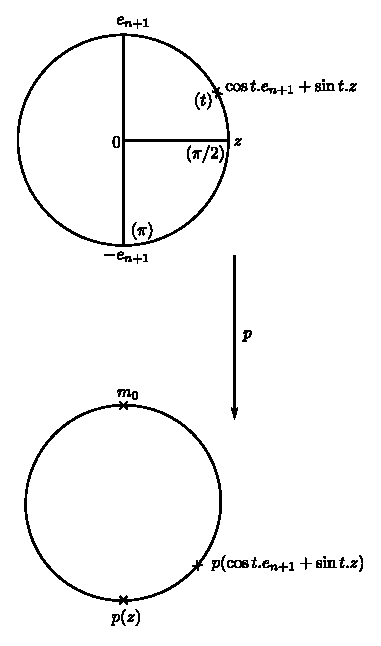
\includegraphics{chap4-fig1.eps}
\end{figure}
\end{proof}

\setcounter{subsection}{4}
\subsection{}\label{chap4:4.5.5}

This result explains the terminology S.C.-manifolds (S.C. stands for
``symmetric circled'').

\subsection{}\label{chap4:4.5.6}

\begin{remark*}
In $(\mathbb{S}^{d},\can)$ two geodesics through $m\in\mathbb{S}^{d}$
meet again at the first time at the antipodal point $-m$ of
$\mathbb{S}^{d}$. For the other S.C.-manifolds the situation will be
described in the proposition below; in its statement in the case of
$P^{2}(\Gamma)$ one should replace ``$z$, $z'$ are or not
$K$-dependent'' by the following: ``$z$, $z'$ \pageoriginale belong or
not to the same fibre of the canonical fibration $\mathbb{S}^{15}\to
\mathbb{S}^{8}$''. 
\end{remark*}

\subsection{}\label{chap4:4.5.7}

\begin{prop*}
Let $(M,g)$ be an S.C.-manifold other than an $(\mathbb{S}^{d},\can)$;
then two geodesics through $m_{0}$ with tangent vectors $p^{T}(r(z))$,
$p^{T}(r(z'))$ at $m_{0}$ (for $z$, $z'\in K^{n}$, $<z,z>=<z',z'>=1$
and $z'\neq \pm z$)
\begin{itemize}
\item[i)] never meet except at $m_{0}$ if $z$, $z'$ are
  $K$-independent

\item[ii)] meet exactly at $m_{0}$ and at their mid-point at distance
  $\dfrac{\pi}{2}$ if $z$, $z'$ are $K$-dependent.
\end{itemize}
\end{prop*}

\begin{proof}
By the argument in the proof of (\ref{chap4:4.5.4}) our two geodesics meet
at distances $t$, $t'$ from $m_{0}$ if and only if
$\exists\,\lambda\in K$ such that
$$
\cos t.e_{n+1}+\sin t.z=\lambda(\cos t'\cdot e_{n+1}+\sin t'\cdot z')
$$
hence
$$
\cos t=\lambda\cdot \cos t'\quad\text{and}\quad \sin t.z=\lambda\cdot
\sin t'\cdot z'.
$$
We can suppose that $t$, $t'\in ]0$, $\pi[$. Since $|\lambda|=1$
    either $\cos t=\cos t'=0$ or $\lambda\in\mathbb{R}$. In the first
    case $t=t'=\dfrac{\pi}{2}$ and $z=\lambda\cdot z'$ so $z$, $z'$
    are $K$-dependent. In the second $\lambda\in \mathbb{R}$,
    $<z,z>=<z',z'>=1$ and $\sin t\cdot z=\lambda\cdot \sin t'\cdot z$
    would imply $z=\pm z'$, a contradiction.
\end{proof}

\begin{remark*}
For $P^{d}(\mathbb{R})$ in fact $z\neq \pm z'$, implies $z$, $z'$ are
never $\mathbb{R}$-dependent so two distinct geodesics in
$P^{d}(\mathbb{R})$ meet at most at one point as they should since
they are projective lines.
\end{remark*}

\setcounter{subsection}{11}
\subsection{}\label{chap4:4.5.12}

\begin{prop*}
For every point $m$ of an S.C.-manifold $(M,g)$ we have
\begin{enumerate}
\renewcommand{\labelenumi}{\theenumi)}
\item $\exp_{m}$\pageoriginale is $\pi$-O.K. if $(M,g)$ is an
  $(\mathbb{S}^{d},\can)$

\item $\exp_{m}$ is $\dfrac{\pi}{2}$-O.K. in the other cases.
\end{enumerate}
\end{prop*}

\begin{proof}
By (\ref{chap4:4.5.6}) we see that for $M=\mathbb{S}^{d}$, $\exp_{m_{0}}$
is one-one on. $\underbar{B}(m_{0},\pi)$ and if $M\neq \mathbb{S}^{d}$
by (\ref{chap4:4.5.7}) that $\exp_{m_{0}}$ is one-one on
$\underbar{B}(m_{0},\dfrac{\pi}{2})$. Thus it suffices to show that
$\exp_{m_{0}}$ is of maximal rank on $\underbar{B}(m_{0},\pi)$ in the
case of $\mathbb{S}^{d}$ and on $\underbar{B}(m_{0},\dfrac{\pi}{2})$
in the other cases. We show, by example for the $P^{n}(K)$'s, that the
  expression we had for geodesics proves in particular that the map
$$
h=\exp_{m_{0}}\circ p^{T}\circ r:K^{n}\to P^{n}(K)
$$
is nothing but
\begin{equation*}
h:tz\to p(\cos t.e_{n+1}+\sin t.z)\quad\text{with}\quad <z,z>=1,
t\in\mathbb{R}.\tag{4.5.13}\label{chap4:4.5.13} 
\end{equation*}
We know that $h^{T}_{tz}(\zeta^{-1}_{tz}z)\neq 0$ by (\ref{chap5:5.6.32}),
and hence we study $h^{T}_{tz}$ for $z'$ with $<z',z'>=1$ and
orthogonal to $z$ in the {\em euclidean} structure of $K^{n}$.

The curve $\alpha\to t(\cos\alpha\cdot z+\sin\alpha\cdot z')$ (whose
speed for $s=0$ is $\zeta^{-1}_{tz}(tz')$) has for image under $h$ the
curve
$$
\alpha\to h(t(\cos \alpha\cdot z+\sin\alpha\cdot z')=p(\cos t\cdot
e_{n+1}+\sin t(\cos \alpha\cdot z+\sin \alpha,z')) 
$$
whose speed for $z=0$ is $p^{T}(\zeta^{-1}_{tz}(\sin t\cdot
z'))$. Since $t\in ]0$, $\dfrac{\pi}{2}[$ and $<z',z'>=1$ one has
  $\sin t\cdot z'.\neq 0$. From $(p^{T})^{-1}(0)\cap K^{n}=\{0\}$ one
  gets the proof.
\end{proof}


\begin{remark*}
(\ref{chap4:4.5.12}) would also follows from (\ref{chap8:8.7.1}).
\end{remark*}

\section{Results of Samelson and Bott}\label{chap4:sec6}

\quad
In the previous article we have seen that in an S.C.-manifold all
geo\-desics are simply closed and of the same length. Now let us examine
the converse. Given a connected riemannian manifold $(M,g)$ such that
for each point $m$ of $(M,g)$
\begin{itemize}
\item[(i)] each \pageoriginale geodesic through $m$ is simply closed;

\item[(ii)] the length of each geodesic through $m$ is a number $1$
  independent of the geodesic; and

\item[(iii)] $1$ is independent of $m$;
\end{itemize}
does it follow that $(M,g)$ is isometric with an S.C.-manifold? (see
article 8).

More generally we give the:

\subsection{}\label{chap4:defi4.6.1}

\begin{defi*}
Given an r.m.\@ $(M,g)$ and some $m\in M$ we say that $(M,g)$ is a
$C_{m}$-{\em manifold} if it is connected and if all geodesics through
$m$ are simply closed and of same length.
\end{defi*}

Though there are no isometry relations between an arbitrary
$C_{m}$-manifold and an S.C.-manifold we shall see that the cohomology
ring of a $C_{m}$-manifold resembles that of an S.C.-manifold. Let us
recall some definitions and results from algebraic topology.

Given a compact topological manifold $M$ we denote its graded
cohomology ring over a ring A by $H^{\ast}(M,A)$.

\subsection{}\label{chap4:4.6.2}

\begin{defi*}
The manifold $M$ is said to be a $TR(A)$-{\em manifold} if
$H^{\ast}(M,A)$ is a truncated polynomial ring.
\end{defi*}

This means $H^{\ast}(M,A)$ is isomorphic to $A[X]/\mathfrak{A}$ where
$\mathfrak{A}$ is an ideal generated by a positive power of $X$. The
image under that isomorphism of $X$ is a homogeneous element of
$H^{\ast}(M,A)$; call its degree $\alpha$. If $d=\dim M$, then define
$\lambda$ by $d=\alpha\cdot \lambda$. The following results are
standard.
\begin{equation*}
\begin{split}
& \mathbb{S}^{d}\text{ is a } TR(\mathbb{Z})\text{ manifold with
  }\alpha=d\text{ and }\lambda=1\\
& P^{n}(\mathbb{C})\text{ is a } TR(\mathbb{Z})\text{  manifold with }
  \alpha=2 \text{ and } \lambda=n\\
& P^{n}(\mathbb{H})\text{ is a } TR(\mathbb{Z})\text{ manifold with }
  \alpha=4\text{ and }\lambda=n\\
& P^{2}(\Gamma)\text{ is a } TR(\mathbb{Z})\text{ manifold with
  }\alpha=8\text{ and } \lambda=2\\
& P^{d}(\mathbb{R})\text{ is a } TR(\mathbb{Z}_{2})\text{ manifold
    with } \alpha=1\text{ and }\lambda=d.
\end{split}\tag{4.6.3}\label{chap4:4.6.3}
\end{equation*}\pageoriginale
We shall prove a result due to Samelson to the effect that a
$C_{m}$-manifold is a $TR(\mathbb{Z}_{2})$-manifold.

\setcounter{subsection}{3}

\subsection{}\label{chap4:4.6.4}

\begin{remark*}
In the definition of a $C_{m}$-manifold we have assumed that all the
geodesics through $m$ are of the same length. This property is not a
consequence of the former namely that each geodesic is simply
closed. To see this one can take either a suitable lens space or more
precisely the following example due to I.M.\@ Singer. A compact Lie
group $G$ is always a symmetric space, when associated to the
symmetric pair $(G\times G,G)$ for the involutive automorphism
$\sigma(g,h)=(h,g)$. For r.s.\@ as in (\ref{chap3:sec3}) the geodesics
through $e$ are the one-parameter subgroups (as follows from
(\ref{chap4:4.4.1})). Take now $G=S0(3)$ and such an r.s.\@ on it; if
$H$ is the subgroup generated by an element of order two then the
quotient $G/H$ is endowed with an r.s.\@ by (\ref{chap3:sec3}), which makes
$G\to G/H$ a riemannian covering. Then the geodesics through $p(e)$
are all of same length (as in $S0(3)$) with one exception (the one
which corresponds to that in $S0(3)$ which contains $H$) which is of
length half that of the others.
\end{remark*}

However \pageoriginale it is not known whether the assumption of equal 
length is, or is not, superfluous in the case of {\em simply
  connected} manifolds.


\subsection{}\label{chap4:4.6.5}

\begin{prop*}
Let $(M,g)$ be a $C_{m}$-manifold for which the (common)\break length of the
geodesics through $m$ equals $1$. Then,
\begin{enumerate}
\renewcommand{\labelenumi}{\theenumi)}
\item $\Omega\supset T_{m}(M)$ and
  $M=\exp(\overline{\underbar{B}(m,1/2)})$ in (particular $M$ is
  compact)

\item if $\dim M\geq 2$, then:either $M$ is simply connected, or the
  universal riemannian covering $(\widetilde{M},\widetilde{g})\to
  (M,g)$ is two-sheeted and $(\widetilde{M},\widetilde{g})$ is a
  $C_{\widetilde{m}}$-manifold $\forall \widetilde{m}\in p^{-1}(m)$,
  with common length for the geodesics through $\widetilde{m}$ equal
  to 21.
\end{enumerate}
\end{prop*}

\begin{proof}
Because each geodesic is of length $1$ we have
$$
\underbar{B}(m,\frac{1}{2})\subset \Omega.
$$
Since every geodesic, and hence $\exp_{m}$, is periodic with period
$1$ we have
$$
T_{m}(M)\subset \Omega.
$$
Since $M$ is connected the Hopf-Rinow theorem (\ref{chap4:4.4.1}) implies
that $M=\exp(T_{m}(M))$. Now the periodicity of $\exp_{m}$ implies
that
$$
M=\exp_{m}(T_{m}(M))=\exp_{m}(\overline{\underbar{B}(m,1/2)}).
$$
Since $\overline{\underbar{B}(m,1/2)}$ is a closed ball and hence
compact and $\exp_{m}$ is defferentiable and hence continuous, it
follows that $M$ is compact (for $M$ is Hausdorff). This proves the
first part.
\end{proof}

The \pageoriginale second part of 2) follows from the remark after
(\ref{chap4:4.2.7}). To prove the first part of 2) we remark first that
all the closed geodesics of period $1$ in a $C_{m}$-manifold are
homotopic as loops based at $m$ (hereafter we use notions and
notations of (\ref{chap4:sec6})) if $\dim M\geq 2$; in fact if $\gamma_{1}$,
$\gamma_{2}$ are two such geodesics and $\lambda:[0,1]\to U_{m}(M)$ a
path connecting $\gamma'_{1}(0)$ to $\gamma'_{2}(0)$ in the unit
tangent sphere $U_{m}(M)$ at $m$ then the required homotopy is
\begin{gather*}
(t,\alpha)\to \exp (t\cdot\lambda(\alpha))\\
\text{for}\quad
\exp(0,\lambda(\alpha))=\exp(1\cdot\lambda(\alpha))=m\forall \alpha\in [0,1].
\end{gather*}
In particular the homotopy class in $\pi_{1}(M,m)$ of a closed
geodesic $\gamma$ of period $1$ through $m$ is independent of
$\gamma$, say $a$.\@ moreover $\gamma^{-1}$ is again such a geodesic
and belongs to $a^{-1}$ hence $a=a^{-1}$ or $a^{2}=1$. Now we claim:
any $b\in \pi_{1}(M,m)(b\neq 0)$ is a power of a (which yields the
proposition). In fact let $b\in\pi_{1}(M,m)$, $\widetilde{m}\in
p^{-1}(m)$ and $\widetilde{m}'\neq \widetilde{m}$. By
(\ref{chap4:4.2.7}) the covering $(M,g)$ is complete hence by
(\ref{chap7:7.4.11}) there exists $\widetilde{\gamma}\in
S(\widetilde{m},\widetilde{m}')$. The projection
$\gamma=p\circ\widetilde{\gamma}$ is a geodesic from $m$ to $m$ in
$(M,g)$ so by (\ref{chap4:4.5.2}) has to be a multiple of a closed
geodesic of period $1$ through $m$; hence $b$ is a power of $a$.

\subsection{}\label{chap4:4.6.6}

\begin{theorem*}[H. Samelson.]
$AC_{m}$-manifold is a $TR(\mathbb{Z}_{2})$ manifold.
\end{theorem*}

\subsection{}\label{chap4:4.6.7}


\begin{lemma*}
There exists a positive number $r$ such that
$$
\underbar{B}(m,\frac{1}{2})\cap \exp^{-1}_{m}(B(m,r))=\underbar{B}(m,r).
$$
\end{lemma*}

\begin{proof}
Let \pageoriginale $r'$ be a positive number such that $\exp_{m}$ is 
$r'$-O.K. Then let us set
$$
W=\exp_{m}\left\{\overline{\underbar{B}\left(m,\dfrac{1}{2}\right)}-\underbar{B}(m,r')\right\}.
$$
Note that $\underbar{B}(m,\dfrac{1}{2})-\underbar{B}(m,r')$ is a
closed subset of the compact ball $\underbar{B}(m,\dfrac{1}{2})$ and
hence compact. Therefore $W$ is compact. Since the geo\-desics through
$m$ are {\em simply} closed it follows that $m\not\in W$. Hence there
is a positive number $r$ such that
\begin{itemize}
\item[i)] $0<r<r'$ and

\item[ii)] $B(m,r)\cap W=\emptyset$.
\end{itemize}
Now let $n\in B(m,r)$ and let $n=\exp_{m}(x)$ where
$||x||<\dfrac{1}{2}$. Since $B(m,r)\cap W=\emptyset$ we see that
$x\not\in \underbar{B}(m,\dfrac{1}{2})-\underbar{B}(m,r')$ and hence
$x\in\underbar{B}(m,r')$. But since $\exp_{m}$ is $r'$-O.K. and $r<r'$
we have $\exp_{m}$ is one-one on $\underbar{B}(m,r)$ and since $n\in
B(m,r)$ we have $x\in\underbar{B}(m,r)$.
\begin{figure}[H]
\centering
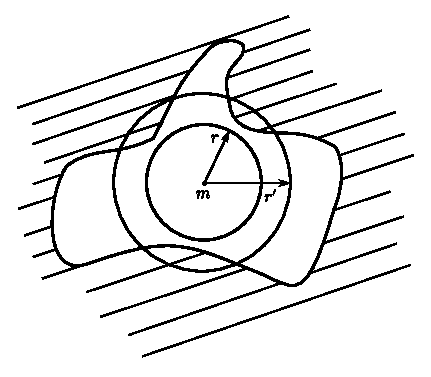
\includegraphics{figures/chap4-fig2.eps}
\end{figure}
\end{proof}

\noindent
{\bf Proof of the proposition.}~By (\ref{chap4:4.5.4}) we can multiply the
r.s.\@ on $(P^{d}(\mathbb{R}),\unskip\break\can)$ by a constant so as to make the
common length of its geodesics equal to $1$, the length of each closed
geodesic of $(M,g)$ through \pageoriginale $m$. Let us fix a point $n$
on $P^{d}(\mathbb{R})$ and a euclidean isomorphism
$$
u:T_{n}(P^{d}(\mathbb{R}))\to T_{m}(M).
$$
Now we {\em define a map} $f\in D(P^{d}(\mathbb{R}),M)$ by requiring
the commutativity of the diagram:
\[
\xymatrix@=1.5cm{
\overline{\underbar{B}(n,\dfrac{1}{2})}\ar[d]_{\exp}\ar[r]^{u} &
T_{m}(M)\ar[d]^{\exp}\\
P^{d}(\mathbb{R})\ar[r]_{f} & M
}
\]
By (\ref{chap4:4.5.12}) $\exp_{n}$ is $\dfrac{1}{2}$-O.K.\@ and hence
the map
$$
\exp_{m}\circ u\circ (\exp_{n}|\underbar{B}(n,\dfrac{1}{2}))^{-1}
$$
is well defined on $B(n,\dfrac{1}{2})$. On $B(n,\dfrac{1}{2})$ we
define $f$ to be this map. Now let $n'\in
\exp(\underbar{B}(n,\dfrac{1}{2})-B(n,\dfrac{1}{2}))$. Then if
$x\in - \,B(n,\dfrac{1}{2})$ and $\exp x=n'$, since the length
of every geodesic is equal to $1$ we have $\exp(-x)=n'$. By
(\ref{chap4:4.5.7}) no two geodesics through $n$ meet outside $n$ and
hence it follows $\pm x$ are the only inverse images of $n'$ in 
$$
\overline{\underbar{B}(n,\dfrac{1}{2})}-B(n,\dfrac{1}{2}).
$$
Since\pageoriginale
$$
||u(x)||=||u(-x)||=\dfrac{1}{2}
$$
and since the common length of geodesics through $m$ is $1$, we
conclude that
$$
\exp(u(x))=\exp(u(-x)).
$$
Now, we extend $f$ to $\underbar{B}(n,\dfrac{1}{2})$ by setting
$$
f(x)=\exp(u(x)).
$$
By \eqref{chap4:4.5.13} $f$ is a differentiable map. (We need only the fact
that $f$ is continuous). Now we claim that the topological degree
$\mod 2$ of $f$ is one. First let us recall the process of getting the
topological degree of a map.

First we can define the fundamental class $\mod 2$ of the compact
manifold $M$ as follows.

We pick up a neighbourhood $U$ of an arbitrary point $m$ of $M$ such
that $U$ is homeomorphic to an open ball. Then we consider the exact
sequence
$$
0\to
H^{d}_{c}(U,\mathbb{Z}_{2})\xrightarrow{i}H^{d}(M,\mathbb{Z}_{2})\to
H^{d}(X-U,\mathbb{Z}_{2})\to\cdots 
$$

(\cite{12}: p. 190. th. 4.10.1 and the following lines), in which
$H^{d}_{c}(U,\mathbb{Z}_{2})$ consists of exactly two elements $0$ and
$\gamma_{U}$. Then $\varphi_{M}$, the fundamental class $\mod 2$ of
$M$, is $i(\gamma_{U})$. Then, \quad , the degree $\mod 2$ of a map
$$
f:N\to M
$$
from a compact manifold $N$ into $M$ is by definition such that
$$
f^{\ast}(\varphi_{M})=\delta\cdot \varphi_{N}.
$$
In \pageoriginale our case we define $\varphi_{M}$ with the help of the
ball $U=B(m,r)$ given by the lemma and for $N=P^{d}(\mathbb{R})$ and
$\varphi_{N}$ with $U'=B(n,r)$.

Let us note that the lemma together with the definition of $f$ implies
that
$$
f^{-1}(U)=U'
$$
and that $f|U'$ is a diffeomorphism. Then we have (\cite{12}: 4.16.,
p. 199) the following commutative diagram
\[
\xymatrix@C=1.5cm@R=1.2cm{
0\ar[r] & H^{d}_{c}(U)\ar[d]_{f^{\ast}_{c}}\ar[r]^{i} &
H^{d}_{c}(M)\ar[d]^{f^{\ast}}\ar[r] & \cdots\\
0\ar[r] & H^{d}_{c}(U')\ar[r]^{i'} & H^{d}(P^{d}(\mathbb{R}))\ar[r] & \cdots
}
\]
Since $f:U'\to U$ is a homeomorphism we have
$$
f^{\ast}(\gamma_{U})=\gamma_{U'}.
$$
Since $\varphi_{M}=i(\gamma_{U})$ and $\varphi_{N}=i'(\gamma_{U'})$
the commutativity of the diagram gives
\begin{align*}
(i'\circ f^{\ast}_{c})(\gamma_{U})=i'(f^{\ast}_{c}(\gamma_{U})) &=
  i'(\gamma_{U'})=\varphi_{N}=(f^{\ast}\circ i)(\gamma_{U})=\\
&\quad =f^{\ast}(\varphi_{M})=\delta\cdot \varphi_{M}.
\end{align*}
Hence 
$$
\delta=1.
$$
Now we assert that
$$
f^{\ast}:H^{\ast}(M,\mathbb{Z}_{2})\to
H(P^{d}(\mathbb{R}),\mathbb{Z}_{2})
$$
is injective. For \pageoriginale Poincar\'e duality asserts that given
any non-zero $e\in H^{\ast}(M,\mathbb{Z}_{2})$, $\exists\, e'\in
H^{\ast}(M,\mathbb{Z}_{2})$ such that
$$
e\cup e'=\varphi_{M}.
$$
Hence we have
$$
f^{\ast}(e)\cup f^{\ast}(e')=f^{\ast}(e\cup
e')=f^{\ast}(\varphi_{M})=\varphi_{N}
$$
and hence
$$
f^{\ast}(e)\neq 0\forall e\quad\text{i.e.}\quad f^{\ast}\quad\text{is
  injective.}
$$
Hence $H^{\ast}(M,\mathbb{Z}_{2})$ is isomorphic to a homogeneous
sub-ring $A$ of the truncated polynomial ring
$$
H^{\ast}(P^{d}(\mathbb{R}),\mathbb{Z}_{2})=\mathbb{Z}_{2}[X]/(X^{d+1})\quad\text{(by
\eqref{chap4:4.6.3}).}
$$
Let $\overline{X}$ be the image of $X$ in
$H^{\ast}(P^{d}(\mathbb{R}),\mathbb{Z}_{2})$ and
$\overline{X}^{\theta}$ be the least positive power of $\overline{X}$
that is in $A$. Then $\exists\, e'\in H^{\ast}(M,\mathbb{Z}_{2})$ such
that $\overline{X}^{\theta}=f^{\ast}(e')$ and by Poincar\'e duality
$\exists\, e'_{1}\in H^{\ast}(M,\mathbb{Z}_{2})$ such that $e'\cup
e'_{1}=\varphi_{M}$. Hence $f(e'_{1})=\overline{X}^{d-\theta}\in
A$. By the same token, for $k$ with $d>k^{\theta}$ we have
$\overline{X}^{k\theta}\in A$ and $\overline{X}^{d-k^{\theta}}\in
A$. So the choice of $\theta$ implies $\exists\, k|d=k\cdot\theta$ and
$H(M,\mathbb{Z}_{2})$ is isomorphic to the truncated polynomial ring
$\mathbb{Z}_{2}[X]/(X^{k+1})$.

\setcounter{subsection}{8}
\subsection{}\label{chap4:4.6.9}

\begin{remark*}
In fact Samelson's result is sharper. But by using Morse theory Bott
proved the following theorem:
\end{remark*}


\subsection{}\label{chap4:4.6.10}

\begin{theorem*}[\cite{6}: p.375]
A simply connected $C_{m}$-manifold is a
$TR(\mathbb{Z})$-mani\-fold. The universal covering of an r.m.\@ which
is not simply connected is a homotopy sphere.
\end{theorem*}

We \pageoriginale will not go into the proof of this theorem but be
content with the remark that recent theorems in algebraic topology and
\eqref{chap4:4.6.3} imply the following: 
\begin{enumerate}
\renewcommand{\labelenumi}{\theenumi)}
\item For a simply connected $TR(\mathbb{Z})$-manifold the cohomology
  $\ring H^{\ast}\unskip\break (M,\mathbb{Z})$ is isomorphic to that of an
  S.C. manifold.

\item a simply connected $C_{m}$-manifold of dimension $d$ odd and
  $d>5$ is homeomorphic to $\mathbb{S}^{d}$.

\item a $C_{m}$-manifold, of dimension greater than or equal to 5 and
  which is not simply connected is homeomorphic to $P^{d}(\mathbb{R})$.
\end{enumerate}

\section{Expressions for $G$ in local coordinates}\label{chap4:chap4-sec7}

Given $(M,g)$ let us express $G$, locally, in terms of $g$. Let us
follow the conventions of (\ref{chap0:sec4}).

On $T(U)$ let us set
\begin{equation*}
G^{\bigdot}=(g^{\sharp})^{T}\circ G\circ g^{\flat}\quad\text{and compute
} G^{\bigdot}.\tag{4.7.1}\label{chap4:4.7.1}
\end{equation*}
Now for
$$
\omega=(x^{1},\ldots,x^{d};p_{1},\ldots,p_{d})\in T^{\ast}(U)
$$
let
\begin{equation*}
G^{\bigdot}(\omega)=(x^{1},\ldots,x^{d};p_{1},\ldots,p_{d};v^{1},\ldots,v^{d};w_{1},\ldots,w_{d}).\tag{4.7.2}\label{chap4:4.7.2} 
\end{equation*}
Let $\{Y_{1},\ldots,Y_{d};P^{1},\ldots,P^{d}\}$ be the basis of
$\mathscr{C}(T^{\ast}(U))$ dual to the basis
$dx^{1},\ldots,dx^{d};dp_{1},\ldots,dp_{d}$ of
$\mathscr{C}^{\ast}(T^{\ast}(U))$.

Now set
\begin{equation*}
H=\frac{1}{2}E\circ g^{\flat}.\tag{4.7.3}\label{chap4:4.7.3}
\end{equation*}
Then by the definition of $G$ we have
$$
i(G^{\bigdot})(d\mu)=-dH.
$$
Hence\pageoriginale
\begin{align*}
d\mu(G^{\bigdot},Y_{i}) &=-\dfrac{\partial H}{\partial
  x^{i}}\tag{4.7.4}\label{chap4:4.7.4}\\
d\mu(G,P^{i}) &= -\dfrac{\partial H}{\partial p_{i}}\tag{4.7.5}\label{chap4:4.7.5} 
\end{align*}
and hence by \eqref{chap0:0.4.26} we have
\begin{align*}
v^{i} &= \frac{\partial H}{\partial p_{i}}\tag{4.7.6}\label{chap4:4.7.6}\\
w_{i} &= \frac{\partial H}{\partial x^{i}}\tag{4.7.7}\label{chap4:4.7.7}
\end{align*}
Now we compute $G$ on $U$. By the definition of $g^{\sharp}$ we have
\begin{equation*}
g^{\sharp}(x^{1},\ldots,x^{d};p^{1},\ldots,p^{d}) =
(x^{1},\ldots,x^{d};p_{1},\ldots,p_{d})\tag{4.7.8}\label{chap4:4.7.8}  
\end{equation*}
where
$$
p_{i}=\sum_{j}g_{ij}p^{j}\quad\text{(see (\ref{chap3:sec8}))}. 
$$
Now let
\begin{gather*}
(g^{\sharp})^{T}(x^{1},\ldots,x^{d};p^{1},\ldots,p^{d};v^{1},\ldots,v^{d};w^{1},\ldots,w^{d})=\tag{4.7.9}\label{chap4:4.7.9}\\
=(x^{1},\ldots,x^{d};p_{1},\ldots,p_{d};v^{1},\ldots,v^{d};w_{1},\ldots,w_{d}). 
\end{gather*}
Then a straightforward calculation of the Jacobian $Dg^{\sharp}$ gives
that
\begin{equation*}
w_{1}=\sum_{i,k}\frac{\partial g_{ij}}{\partial x^{k}}\cdot v^{k}\cdot p^{j}+\sum_{j}g_{ij}w^{j}.\tag{4.7.10}\label{chap4:4.7.10}
\end{equation*}
Now let
{\fontsize{9}{11}\selectfont
$$
G(x^{1},\ldots,x^{d};p^{1},\ldots,p^{d})=(x^{1},\ldots,x^{d};p^{1},\ldots,p^{d};p^{1},\ldots,p^{d};G^{1},\ldots,G^{d}).
$$}\relax
With the notation of (\eqref{chap1:1.3.2}) we have
\begin{equation*}
G^{i}=-\sum_{j,k}\Gamma^{i}_{jk}p^{j}p^{k}.\tag{4.7.11}\label{chap4:4.7.11}
\end{equation*}\pageoriginale
Hence we have to compute $\Gamma^{i}_{jk}$. We have
{\fontsize{9}{11}\selectfont
$$
G(x^{1},\ldots,x^{d};p_{1},\ldots,p_{d}) =
(x^{1},\ldots,x^{d};p_{1},\ldots,p_{d};p^{1}, \ldots,p^{d};
G_{1},\ldots,G_{d}).  
$$}\relax
From \eqref{chap3:3.8.3} it follows that
\begin{equation*}
H=\frac{1}{2}\sum_{j,k} g^{jk}p_{j}p_{k}\tag{4.7.12}\label{chap4:4.7.12}
\end{equation*}
and hence
\begin{equation*}
\frac{\partial H}{\partial x^{i}}=\frac{1}{2}\sum_{j,k}\frac{\partial
  g^{jk}}{\partial x^{i}}p_{j}p_{k}.\tag{4.7.13}\label{chap4:4.7.13}
\end{equation*}
By \eqref{chap3:3.8.3} we have
$$
\sum_{l}g^{il}g_{lj}=\delta_{ij}
$$
and hence for every $i$
\begin{equation*}
\sum_{j,k}\frac{\partial g^{jk}}{\partial
  x^{i}}p_{j}p_{k}=-\sum_{j,k}\frac{\partial g^{jk}}{\partial
  x^{i}}p^{j}p^{k}.\tag{4.7.14}\label{chap4:4.7.14} 
\end{equation*}
Hence by \eqref{chap4:4.7.7}, \eqref{chap4:4.7.10} and \eqref{chap4:4.7.14} we have
\begin{equation*}
\sum_{j,k}\frac{\partial g_{ij}}{\partial
  x^{k}}p^{k}p^{j}+\sum_{j}g_{ij}G^{j}=\frac{1}{2}\sum_{j,k}\frac{\partial
  g_{jk}}{\partial x^{i}}p^{j}p^{k},\tag{4.7.15}\label{chap4:4.7.15}
\end{equation*}
or
\begin{equation*}
\sum_{j}g_{ij}G^{i}+\sum_{j,k}\frac{1}{2}\left(2\frac{\partial
  g_{ij}}{\partial x^{k}}-\frac{\partial g_{ik}}{\partial
  x^{i}}\right)p^{j}p^{k}=0.\tag{4.7.16}\label{chap4:4.7.16} 
\end{equation*} 
Now \pageoriginale if we set
\begin{equation*}
\Gamma_{jik}=\frac{1}{2}\left(\frac{\partial g_{ij}}{\partial
  x^{k}}+\frac{\partial g_{ik}}{\partial x^{j}}-\frac{\partial
  g_{jk}}{\partial x^{i}}\right)\tag{4.7.17}\label{chap4:4.7.17}
\end{equation*}
then we have
\begin{equation*}
\sum_{j}g_{ij}G^{j}+\sum_{j,k}\Gamma_{jik}p^{j}p^{k}=0.\tag{4.7.18}\label{chap4:4.7.18}
\end{equation*}
Hence by the definition of $g^{ij}$ we have
\begin{equation*}
\Gamma^{i}_{jk}=\sum_{l}g^{il}\Gamma_{jlk}\tag{4.7.19}\label{chap4:4.7.19}
\end{equation*}
where the $\Gamma_{jlk}$ are given by \eqref{chap4:4.7.17}.

\begin{remark*}
\eqref{chap4:4.7.6} and \eqref{chap4:4.7.7} are nothing but Hamilton's
equations. 
\end{remark*}

\subsection{Lagrange's equation}\label{chap4:4.7.20} 

In local coordinates \eqref{chap4:4.2.1} also yields Lagrange's
equations. On $T(U)$ we introduce the local vector fields
\begin{align*}
& \left\{X_{i}=\frac{\partial}{\partial x^{i}}\right\},
  \left\{P_{i}=\frac{\partial}{\partial p^{i}}\right\}\text{ \  and
    have~:}\\
&\qquad
  p^{T}\left(\left[X_{i},G\right]\right)=0,\alpha\left(\left[X_{i},G\right]\right)=0, p^{T}(X_{i})=\xi(p_{i})
\end{align*}
So by (\ref{chap3:3.1.8})
$$
\alpha(X_{i})=\frac{1}{2}\frac{\partial E}{\partial p^{i}}.
$$
And
\begin{gather*}
d\alpha(G,X_{i})=G(\alpha(X_{i}))-X_{i}(\alpha(G))-\alpha([G,X_{i}])=\frac{1}{2}G\left(\frac{\partial
  E}{\partial p^{i}}\right)-X_{i}(E)=\\
=-\frac{1}{2}dE(X_{i})
\end{gather*}
so:\pageoriginale
$$
G\left(\frac{\partial E}{\partial p^{i}}\right)=\frac{\partial
  E}{\partial x^{i}}.
$$
Working along a geodesic parametrized by $t$ implies $G=\dfrac{d}{\dt}$
hence the Lagrange equations:
$$
\frac{d}{\dt}\left(\frac{\partial E}{\partial
  p^{i}}\right)=\frac{\partial E}{\partial x^{i}}.
$$

\section{Zoll's surface}\label{chap4:sec8}

\quad 
In this article we answer negatively the question which was posed at
the beginning of article $6$ by giving a counter example due to Zoll
of a r.s.\@ on $\mathbb{S}^{2}$ for which $\mathbb{S}^{2}$ is a
$C_{m}$-manifold $\forall m\in\mathbb{S}^{-2}$ but not isometric to
$(\mathbb{S}^{2},\can)$.
\begin{center}
\centering
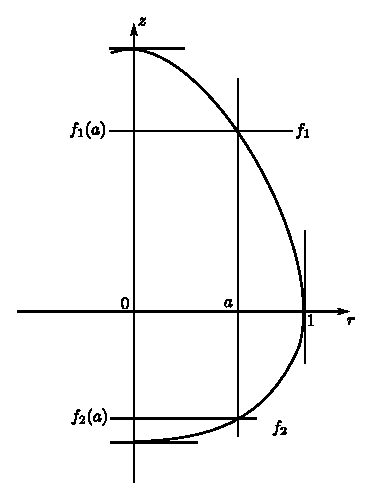
\includegraphics{chap4-fig3.eps}
\end{center}

\noindent
To construct the surface in the $(x,y,z)$-space we take in the
$(z,r)$-plane two curves $r\to f_{i}(r)$ $(i=1,2)$ with $f_{1}$,
$f_{2}\in D([0,1[,\mathbb{R}^{+})$ and\pageoriginale $f_{i}(1)=0$,
    $f'_{i}(0)=0$, $f'_{i}\leq 0$ and $f'_{i}(r)\to
    {\displaystyle{\mathop{\infty}_{1}}}(i=1,2)$.  

We generate a surface of revolution $M$ by setting:
$$
M_{1}=\left\{(x,y,z)|z=f_{1}(\sqrt{x^{2}+y^{2}})\right\},
M_{2}=\left\{(x,y,z)|z=-f_{2}(\sqrt{x^{2}+y^{2}})\right\} 
$$
hence $M=M_{1}\cup M_{2}$ is a $C^{1}$-manifold. We have two charts
$(U_{i},s_{i})(i=1,2)$ on $U_{i}=M_{i}-(z^{-1}(0)\cup (x^{-1}(0)\cap
y^{-1}(0)))$ defined as follows:
\begin{gather*}
\text{if}\quad p(x,y,z)=(x,y)\text{ \ we set}\\
s_{i}(m)=(||p(m)||,\text{ angle } (e_{1},p(m)))\in\mathbb{R}^{2}(i=1,2)
\end{gather*}
(polar coordinates). On $U_{i}$ the local coordinates will be denoted
by $x^{1}=r=u^{1}\circ s_{i}$, $x^{2}=\varphi_{s}=u^{2}\circ s_{i}$
$(i=1,2)$ so that
\begin{equation*}
s^{-1}_{1}(u^{1},u^{2})=(u^{1}\cdot \cos u^{2}, u^{1}\cdot \sin u^{2},
f_{i}(u^{1})).\tag{4.8.1}\label{chap4:4.8.1} 
\end{equation*}
{\em We drop the $i$ in $s_{i}$ and in $f_{i}$.} We have the vector
fields 
\begin{align*}
& \{X_{1},X_{2}\} \text{ \ dual basis of \ } \{dr,d\varphi\}\text{ \  on
  \ } \mathscr{C}(U_{i}),\\
&\{Y_{1},Y_{2}\}\text{ \ dual basis of \ } \{du^{1},du^{2}\} \text{
  \ on \ } \mathscr{C}(\mathscr{R}^{2}).
\end{align*}
We endow $M$ with the r.s.\@ induced by $(\mathbb{R}^{3},\can)$ as in
(\ref{chap3:3.2.1}). For $g=\sum\limits_{i,j}g_{ij}dx^{i}dx^{j}$ we have
by definition of $\epsilon$ (see (\ref{chap3:3.1.2})): 
$$
g_{ij}=g(X_{i},X_{j})=(\zeta\circ (s^{-1})^{T_{\bigdot}}\circ
Y_{i})\cdot (\zeta\circ(s^{-1})^{T}\circ Y_{j})=(Ds^{-1}\circ
Y_{i})\cdot (Ds^{-1}\circ Y_{j})
$$
where $Ds^{-1}$ is the (Jacobian)$^{-1}$ of $s$, i.e. by \eqref{chap4:4.8.1}:
$$
Ds^{-1}=
\begin{pmatrix}
\cos u^{2} & -u^{1}\cdot \sin u^{2}\\
\sin u^{2} & u^{1}\cdot \cos u^{2}\\
f'(u^{1}) & 0
\end{pmatrix}
$$\pageoriginale
hence, setting $f'=\dfrac{df}{dr}$:
\begin{equation*}
g=(1+{f'}^{2})dr^{2}+r^{2}\cdot d\varphi^{2},
g_{12}=1+{f'}^{2},g_{12}=0, g_{22}=r^{2}\tag{4.8.2}\label{chap4:4.8.2}
\end{equation*}
hence by \eqref{chap3:3.8.3}
$$
g^{11}=\dfrac{1}{1+{f'}^{2}}, g^{12}=0, g^{22}=\dfrac{1}{r^{2}};
$$
thus by \eqref{chap4:4.7.17} and \eqref{chap4:4.7.19}:
$$
\Gamma_{122}=r,\Gamma_{121}=\Gamma_{222}=0,
\Gamma_{12}^{2}=\frac{1}{r},\Gamma^{2}_{11}=\Gamma^{2}_{22}=0.
$$
Hence if
$$
\psi:t\to (r(t),\varphi(t))
$$
is a geodesic, then by \eqref{chap1:1.3.5} we have
$$
\frac{d^{2}\varphi}{\dt^{2}}+\frac{2}{r}\cdot \frac{dr}{\dt}\cdot
\frac{d\varphi}{\dt}=0 
$$
i.e.
$$
\frac{d}{\dt}\left(r^{2}\frac{d\varphi}{\dt}\right)=0.
$$
Thus, along a given geodesic, there exists an a such that
\begin{equation*}
r^{2}\frac{d\varphi}{\dt}=a.\tag{4.8.3}\label{chap4:4.8.3}
\end{equation*}
We suppose moreover that $\psi$ is parametrized by arc length, so that
by \eqref{chap4:4.3.3} and \eqref{chap4:4.8.2}:
$$
\left(1+{f'}^{2}\right)\left(\frac{dr}{ds}\right)^{2}+r^{2}\left(\frac{d\varphi}{ds}\right)^{2}=1 
$$\pageoriginale
and hence
$$
\left|\frac{d\varphi}{ds}\right|\leq \frac{1}{r}.
$$
Now by \eqref{chap4:4.8.3} we have
$$
a\leq \frac{1}{r(s)}\cdot r^{2}(s)=r(s),
$$
and hence the geodesic never crosses the curve given by the section of
$M$ by the planes $z=f_{i}(a)$ $(i=1,2)$. Moreover:
\begin{figure}[H]
\centering
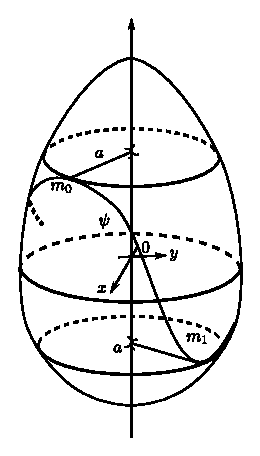
\includegraphics{figures/chap4-fig5.eps}
\end{figure}
\begin{equation*}
\frac{d\varphi}{dr}=\frac{a}{r}\left(\frac{1+{f'}^{2}}{r^{2}-a^{2}}\right)^{1/2}.\tag{4.8.4}\label{chap4:4.8.4}
\end{equation*}

\setcounter{subsection}{4}
\subsection{}\label{chap4:4.8.5}
Let\pageoriginale us note that (by continuity arguments, for our
computations are not valid outside $U_{1}\cup U_{2}$) that the
geodesics corresponding to $a=0$ are the meridians and that to $a=1$
corresponds the equator. So to ensure that $M$ is a $C_{m}$-manifold
$\forall m\in M$ we have only to take care of the case $0<a<1$. Let
then $m_{0}=(x_{0},y_{0},f_{1}(a))$ and $m_{1}=x_{1},y_{1},-f_{2}(a)$)
be extreme points of $\psi$ such that the part of $\psi$ between them
does not meet again the planes $z=f_{1}(a)$, $z=-f_{2}(a)$. Then -
thanks to the symmetry of $M$-showing that $\psi$ is simply closed
amounts to showing that the variation $\Phi(a)$ of the angle $\varphi$
from $m_{0}$ to $m_{1}$ is equal exactly to $\pi$. Since the integral
$$
\int\limits^{1}_{a}\frac{a}{r}\left(\frac{1+{f'}^{2}}{r^{2}-a^{2}}\right)^{1/2}\cdot
dr
$$
exists we have by \eqref{chap4:4.8.4} applied for the part of $\psi$ in
$U_{1}$ and for the part in $U_{2}$:
\begin{equation*}
\Phi(a)=\int\limits^{1}_{a}\frac{a}{r}\cdot
\frac{(1+f'_{1})^{1/2}+(1+{f'}^{2}_{2})^{1/2}}{(r^{2}-a^{2})^{1/2}}\cdot dr.\tag{4.8.6}\label{chap4:4.8.6}
\end{equation*}
Then we have shown:

\setcounter{subsection}{6}

\subsection{}\label{chap4:4.8.7}

\begin{theorem*}[Darboux]
The surface $(M,\epsilon|M)$ is a $C_{m}$-manifold $\forall m\in M$ if
and only if $\Phi(a)=\pi \forall a\in ]0$, $1[$, with $\Phi(a)$ as in
    \eqref{chap4:4.8.6}. 
\end{theorem*}

\subsection{}\label{chap4:4.8.8}

\begin{theorem*}[Zoll: \cite{30})]
There exists $f_{1}$, $f_{2}\in D([0,1[,\mathbb{R}^{+})$ such that:
\begin{itemize}
\item[{\rm i)}] $M$ \pageoriginale is a real-analytic sub manifold of
  $\mathbb{R}^{3}$

\item[{\rm ii)}] $M$ is a $C_{m}$-manifold $\forall m\in M$

\item[{\rm ii)}] $M$ is not isometric to $(\mathbb{S}^{2},\can)$.
\end{itemize}
\end{theorem*}

\begin{proof}
A. To find $f_{1}$, $f_{2}$ we derive relations from
$\Phi(a)=\pi\cdot a$. Set
$g=(1+{f'}^{2}_{1})^{1/2}+(1+{f'}^{2}_{2})^{1/2}$, $\dfrac{1}{r}=x+1$,
$\dfrac{1}{a^{2}}=\alpha + 1$, $x=\alpha\cdot u$, $r\cdot
g(r)=2\cdot\theta(x)$; then we must have 
$$
\int\limits^{\alpha}_{0}\frac{\theta(x)}{(\alpha-x)^{1/2}}\cdot
dx=\pi \,\forall \alpha
$$
and thus
$$
\int\limits^{1}_{0}\frac{\theta(\alpha\cdot
  u)}{(1-u)^{1/2}}\sqrt{\alpha}\cdot du=\pi \, \forall \alpha.
$$
Differentiating the above equation with respect to $\alpha$ we have
\begin{equation*}
\theta(\alpha u)+2\alpha\cdot u\theta'(\alpha u)=0.\tag{4.8.9}\label{chap4:4.8.9}
\end{equation*}
But the function
$$
\theta(x)=\frac{k}{\sqrt{x}}
$$
satisfies the above equation, and since it is known that
$$
\int\limits^{1}_{0}\frac{dx}{(x(1-x))^{1/2}}=\pi
$$
it follows that the function $\dfrac{1}{\sqrt{x}}$ can be taken for
$\theta(x)$. Hence we should try to find $f_{1}$ and $f_{2}$ such
that:
$$
(1+{f'}^{2}_{1})^{1/2}+(1+{f'}^{2})=\frac{2}{\sqrt{(1-r^{2})}}.
$$
(Note that the choice $f_{1}(r)=f_{2}(r)=(1-r^{2})^{1/2}$ makes the
associated surface \pageoriginale a sphere). We set:
$$
(1+{f'}^{2}_{1})^{1/2}=(1-r^{2})^{1/2}+\lambda(r)
$$
and
$$
(1+{f'}^{2}_{2})^{1/2}=(1-r^{2})^{1/2}-\lambda(r)
$$
where in order that the equations have meaning we should have
$$
\frac{1}{1-r^{2}}\pm \lambda(r)\geq 1.
$$
There exist such functions $\lambda$, for example the binomial
expansion of $(1-r^{2})^{1/2}$ gives that the function
$$
k\cdot r^{2}\quad\text{for}\quad 0<k<\frac{1}{2}
$$
is such a function. Hence we set:
\begin{align*}
(1+{f'}^{2}_{1})^{1/2} &= (1-r^{2})^{-1/2}+kr^{2}\\
(1+{f'}^{2}_{2})^{1/2} &= (1-r^{2})^{-1/2}-kr^{2},
\end{align*}
and we know by (\ref{chap4:4.8.7}) that $M$ is a $C_{m}$-manifold
$\forall m\in M$.

B.~We check (i) now. Analyticity has to be checked only at $r=1$ and
we wish to express $r$ as a function of $z$ (instead of $z=f_{1}(r)$,
$z=-f_{2}(r)$). We have (since $f'_{1}<0$, $f'_{2}<0$) and for $z>0$:
$$
\frac{dz}{dr}=f'_{1}=\frac{-r}{\sqrt{(1-r^{2})}}(1+2k(1-r^{2})^{1/2}+k^{2}r^{2}(1-r^{2})) 
$$
so if we set $s=(1-r^{2})^{1/2}$:
$$
\frac{ds}{dz}=\frac{1}{1+2ks+k^{2}s^{2}(1-s^{2})}=b(s)
$$\pageoriginale
with $b(s)$ analytic in $s$. By Cauchy's theorem $\dfrac{ds}{dz}=b(s)$
has a unique analytic solution with $s(0)=0$.

For $z<0$ and $t=-(1-r^{2})^{1/2}$:
$$
-\frac{dz}{dr}=f'_{2}=-\frac{r}{\sqrt{(1-r^{2})}}(1-2k\sqrt{(1-r^{2})}+k^{2}r^{2}(1-r^{2})) 
$$
hence
$$
\frac{\dt}{dz}=\frac{1}{1+2kt+k^{2}t^{2}(1-t^{2})}=b(t)
$$
with the {\em same} $b$. So the unique analytic solution is the same
for $z>0$ and for $z<0$.

C.~We shall prove that $(M,\epsilon|M)$ is not isometric to
$(\mathbb{S}^{2},\can)$. One can either compute the curvature of
$(M,\epsilon|M)$ at a simple point or argue as follows: in
$(\mathbb{S}^{2},\can)$ the meridians are the geodesics. The geodesics
through two antipodal points $m$, $m'$ have a closed geodesic as
orthogonal trajectory, and this geodesic is the locus equidistant from
$m$, $m'$. The same should hold in a surface isometric to
$(\mathbb{S}^{2},\can)$. But for Zoll's surface and the two antipodal
points $m=(0,0,f_{1}(0))$, $m'=(0,0,-f_{2}(0))$ the only orthogonal
trajectory is the equator, which is not equidistant from $m$, $m'$
since the lengths of the meridians from $m$ to the equator and from
the equator to $m'$ are respectively:
\begin{align*}
\int\limits^{1}_{0}(1+{f'}^{2}_{1})^{1/2}dr &=
\int\limits^{1}_{0}(1-r^{2})^{-1/2}dr+\int\limits^{1}_{0}kr^{2}=\overline{2}+\frac{k}{3}\\
\int\limits^{1}_{0}(1+{f'}^{2}_{2})^{1/2}dr &= \int\limits^{1}_{0}(1-r^{2})^{-1/2}dr-\int\limits^{1}_{0}kr^{2}=\overline{2}-\frac{k}{3}.
\end{align*}\pageoriginale
\end{proof}

\setcounter{subsection}{9}

\subsection{}\label{chap4:remas4.8.10}

\begin{remarks*}
A.~Check with the choice $\lambda(r)=\dfrac{3}{2}r^{4}$ that the
meridians have inflexions
\begin{figure}[H]
\centering
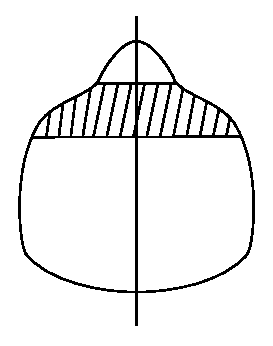
\includegraphics{figures/chap4-fig6.eps}
\end{figure}
So there exist surfaces $(M,\epsilon|M)$ which are $C_{m}$-manifolds
$\forall m\in M$ and which contain points with strictly {\em negative}
curvature (Zoll: \cite{30}). 

B.~We will see (\eqref{chap8:sec9}) the striking fact that if $(M,g)$ is a
$C_{m}$-manifold $\forall m\in M$ for $M$ {\em homeomorphic} to
$P^{2}(\mathbb{R})$ then $(M,g)$ is {\em isometric} to
$(P^{2}(\mathbb{R}),\can)$.

C.~Note \eqref{chap4:4.8.3} is classical for motions with central
acceleration (as it is the case for geodesics of a surface of
revolution since the normal meets the $z$-axis). Note also the
condition
$$
\int\limits^{\alpha}_{0}\frac{\theta(x)}{(\alpha-x)^{1/2}}\cdot
dx=\pi \, \forall \alpha
$$\pageoriginale
is equivalent to the search of tautochronous motions on a vertical
curve and yields the cycloidal pendulum.
\end{remarks*}


